\section{Instance Creation}
In order to test and compare the performance and the quality of the two algorithms, one fundamental step
was to provide some problem instances.
In this section I will describe how I obtained the instances
used as benchmark.
\subsection{Provided Instances}
During the class, the professor provides us two instances, with respectively $12$ and $60$ points.
\subsection{Gerber File}
\label{sec:Gerber}

In order to represent PBCs there is a standard format, that is called \emph{Gerber}, which extension is \verb|.gbr|.
The specification of this file format can be found at: \url{https://www.ucamco.com/files/downloads/file/81/the_gerber_file_format_specification.pdf}. This file format
contains - among a lot of information (such as lines, drill size, interpolation mode, board size, etc.) -
the positions of the drill points.


In order to parse the data from a file in this format, I wrote with my colleague Sebastiano Valle, a parser.
It fetches only the points' position. It can be found in the folder \verb|/GerberParser| and can be opened in each browser, because it is written in javascript and is wrapped into an HTML file, named \verb|index.html|.
You can upload a file using the button "browse" and it returns a \verb|.dat| file containing the euclidean distance between the holes.
The parser tries also to draw the points on the screen, but it works well only with certain instances, because the scale\footnote{You can zoom in and zoom out.} and the center are hard-coded. Therefore in order to view it graphically
you can use this online tool \url{http://www.gerber-viewer.com/}.

One difficulty with this approach was to find real instances for free on the web. I did not succeed, but my brother provided me a real world example file, that I named
\verb|RealWorldExample.gbr|. 
This instance consists of 53 points. It is used as \emph{real-world} example in the chapter about the result \ref{sec:result} and can be viewed in figure \ref{figure:pbc}. 


\begin{figure}[ht!]
	\centering
	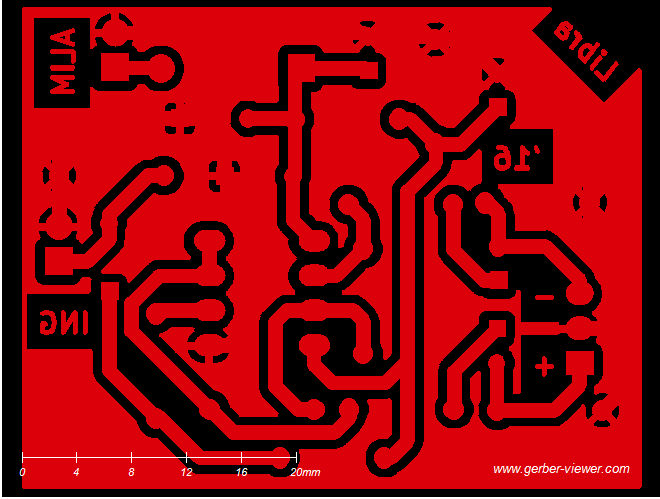
\includegraphics[scale=0.3]{img/real_world.png}
	\caption{The real world example used.}
	\label{figure:pbc}
\end{figure}

\subsection{Instance Generator}
\label{sec:instance:generator}
In order to provide some particular instances, I wrote a program that can be found in the folder
\verb|/InstanceGenerator|. The usage is straightforward: you have to provide N, the number of points and
one letter out of \verb|'r','c','q'| which stands respectively for random, circle, square\footnote{If no option is provided the random option will be considered.}. The board is square-shaped with a fixed side of $10\times N$.
\begin{itemize}
	\item If the option random is provided, it creates randomly $N$ points.
	\item If the option circle is provided, it creates 4 circles of $\lfloor{N/4}\rfloor$ points in the top-left, top-right, bottom-left, bottom-right corner
	of the drill board. If $N\ \text{mod} \ 4 = a$ with $a \neq 0$ then the circles $0\dots a$ will have $\lfloor{N/4}\rfloor + 1$ points.
	\item If the option square is provided, it creates 4 square of $\lfloor{N/4}\rfloor$ points in the top-left, top-right, bottom-left,
	bottom-right corner of the drill board. If $N$ is not a multiple of $4$, it tries to put the extra points somewhere inside the square.
\end{itemize}
In order to visualize the generated instances, the files
\verb!/tmp/tsp_instance_<N>.gbr! and \verb!/tmp/tsp_instance_<N>.pbm!\footnote{This file format is a good choice because it is
portable and easy to encode: 1 bit corresponds to 1 pixel, with 0 = white and 1 = black.} are generated.
The latter file can be opened by each image viewer.
The instance generator program computes a \verb|.dat| file, that contains the costs from each drill point $i$ to each drill point $j$. This file can be used as input for the algorithms.

An example of a square and one circle instance can be found in figure \ref{fig:square_circle}.
These kinds of instances are very similar because the
points are clustered on the corners.
But the circle instances are more flexible because they work well even with N that are not multiple of 4. Therefore they are preferred
over the square ones in the benchmark.
The advantage of the circle instances compared to random generated ones is that the first are reproducible and the second are not.


\begin{figure}[h!]
	\centering
	\fbox{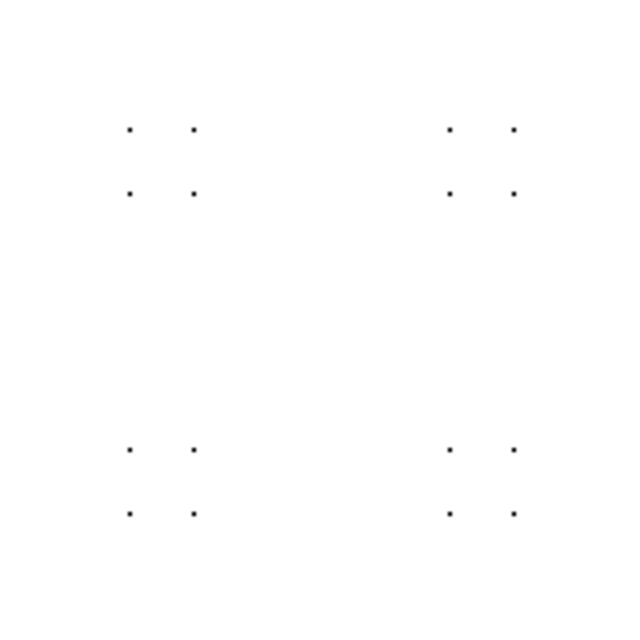
\includegraphics[scale=0.23]{img/square.png}}
	\fbox{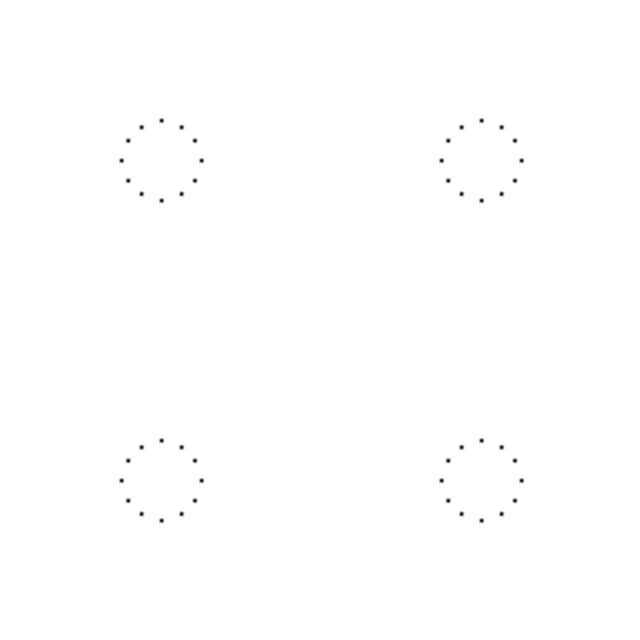
\includegraphics[scale=0.23]{img/circle.png}}
	\caption{A sample square instance with 16 holes circle instance with 48 holes.}
	\label{fig:square_circle}
\end{figure}